\subsubsection{Korekcja (patching) linii (Win32)}

Możemy w łatwy sposób znaleźć linię ``hello, world'' w pliku wykonywalnym za pomocą Hiew:

\begin{figure}[H]
\centering
\myincludegraphics{patterns/01_helloworld/hola_edit1.png}
\caption{Hiew}
\label{}
\end{figure}

Możemy przetłumaczyć naszą wiadomość na jeżyk hiszpański:

\begin{figure}[H]
\centering
\myincludegraphics{patterns/01_helloworld/hola_edit2.png}
\caption{Hiew}
\label{}
\end{figure}

Tekst w języku kiszpańskim jest o 1 bajt krótszy od tekstu w języku angielskim, dlatego dodajemy na koniec bajt 0x0A (\TT{\textbackslash{}n}) i bajt zerowy.
Działa.

A co jeśli chcemy wstawić dłuższe powiadomienie?
Po oryginalnym tekście w j. angielskim widzimy jakieś bajty zerowe.
Ciężko powiedzieć, czy można je nadpisać: mogą one być wykorzystywane gdzieś w \ac{CRT}-kodzie, a mogą i nie być.
Tak czy inaczej, możemy je nadpisywać tylko jeśli naprawdę wiemy co robimy.

\subsubsection{Korekcja linii (Linux x64)}

\myindex{\radare}
Spróbujmy spatchować plik wykonywalny dla Linux x64 korzystając z \radare{}:

\lstinputlisting[caption=Sesja w \radare{}]{patterns/01_helloworld/radare.lst}

Co się tu dzieje: szukam linii \q{hello} korzystając z komendy \TT{/}, 
zatem ustawiam \emph{kursor} (\emph{seek} w terminach \radare{}) pod ten adres.
Następnie chcę się upewnić, że jest to rzeczywiście potrzebne miejsce: \TT{px} wylistowuje bajty pod tym adresem.
\TT{oo+} przełącza \radare{} w tryb \emph{odczytu-zapisu}.
\TT{w} zapisuje ASCII-linię w miejscu kursora (\emph{seek}).
Warto zauważyć, iż \TT{\textbackslash{}00} na końcu jest bajtem zerowym.
\TT{q} kończy pracę.

% TBT
%\subsubsection{This is a real story of software cracking}
%\label{\SoftwareCracking}
%
%An image processing software, when not registered, added watermarks,
%like ``This image was processed by evaluation version of [software name]'', across a picture.
%We tried at random: we found that string in the executable file and put spaces instead of it.
%Watermarks disappeared.
%Technically speaking, they continued to appear.
%\myindex{Qt}
%With the help of Qt functions, the watermark was still added to the resulting image.
%But adding spaces didn't alter the image itself...

\subsubsection{Lokalizacja oprogramowania za czasów MS-DOS}

Sposób przedstawiony wyżej był rozpowszechniony przy tłumaczeniu oprogramowania pod MS-DOS na język rosyjski w latach 80 i 90.
Rosyjskie słowa i zdania zwykle dą trochę dłuższe od odpowiedników w j. angielskim, dlatego \emph{lokalne} oprogramowanie zawierało 
sporo dziwnych akronimów i ciężkich w zrozumieniu skrótów.

\begin{figure}[H]
\centering
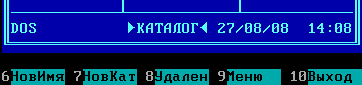
\includegraphics[width=0.5\textwidth]{patterns/01_helloworld/Norton_Commander_v5_51.png}
\caption{\PLph{}}
\end{figure}

Prawdopodobnie, sytuacja wyglądała podobnie z tłumaczeniem na inne języki.

